\documentclass[11pt,a4paper]{article}
%\documentclass[conference]{IEEEtran}
\usepackage[english]{babel} 
\usepackage[T1]{fontenc}
\usepackage{lmodern}
\usepackage[utf8]{inputenc}
\usepackage{eurosym}
\DeclareUnicodeCharacter{20AC}{\euro}
\usepackage{graphicx}
\usepackage{rotating} 
\usepackage{array}
\usepackage{booktabs} 
\usepackage{longtable}
\usepackage{ifthen}
\usepackage{xcolor}
\usepackage{tabu}
\usepackage{colortbl}
\usepackage{calc}
\usepackage{pifont}
\usepackage{forloop}
\usepackage[nomessages]{fp}

\usepackage{amsmath}
\usepackage{amssymb}
\usepackage{amsthm} 

\newtheoremstyle{break}
   {\topsep}{\topsep}%
   {\itshape}{}%
   {\bfseries}{}%
   {\newline}
   {\thmname{#1}\thmnumber{\@ifnotempty{#1}{ }\@upn{#2}}%
    \thmnote{ {\bfseries(#3)}}}% 
    
\newtheorem{definition}{Definition}

\usepackage[parfill]{parskip}
%\usepackage[onehalfspacing]{setspace}
\usepackage{newclude}

\newcounter{starnumber}
\newcommand{\stars}[1]{
  \forloop{starnumber}{1}{\value{starnumber} < 6}{
    \ifthenelse{#1 < \value{starnumber}}{\ding{73}}{\ding{72}}%
  }
}

\renewcommand{\arraystretch}{1.2}

%\usepackage[sortcites=true, style=authoryear,natbib=true]{biblatex}
\usepackage{biblatex}
\bibliography{bibliography}

%Autornamen in Bibliography fett
%\AtBeginBibliography{\renewcommand*{\mkbibnamelast }[1]{\textbf{#1}}}
%\AtBeginBibliography{\renewcommand*{\mkbibnamefirst }[1]{\textbf{#1}}}

%\makeindex

\title{Development of a educational and sustainable robotic platform for children and adults}
\date{\today}
\author{Sebastian Muszytowski \\Baden-Wuerttemberg Cooperative State University Mannheim }

\begin{document}

\maketitle
%\twocolumn[
%       \maketitle
%        \begin{@twocolumnfalse}
%        \maketitle
%        \end{@twocolumnfalse}
%]


\section{Introduction}
Getting children in touch with technology is important in todays technologically advanced society. In schools technology (specifically electrical engineering and programming) is often taught using robots. Robots are well suited for children since they allow interaction with the reality in contrast to arbitrary technology related exercises such as programming exercises which doesn't affect the real world.\newline 
Since schools are required to save money, robots used for teaching stay property of the schools. Therefore children usually cannot take the robot home to work with it. In addition modification of robot is usually not permitted which reduces potential learning experiences. Giving students the full control over all possibilities of the robot requires them to own the robot. This requires to robot to be cheap, extendable and suitable for educational purposes.\newline
The development of a robot platform for educational purpose requires requirement engineering, market research and evaluation of robots which are already used in education. Once the research is completed a new robot platform can be constructed taking the research results into account.
\section{Requirement Analysis / Project Goals}
The target user group of the robot are mainly children and adults with very little or no experience in electrical engineering and programming. Teaching the knowledge requires a platform which is designed to be educational. Therefore it has to comply with several requirements which affect technical aspects as well as social aspects.
The following lists describes the basic requirements on which existing platforms can be assessed. The assessment criteria can also be used to make decisions when developing a new platform.
\begin{description}
\item[Affordable] \hfill \\ The robot platform must be affordable for everyone. Especially when the robot is used in schools every child should own the robot to increase the possibilities to modify and extend it. Robots which stay property of a school may result in social problems since socially disadvantaged children cannot afford their own robot whereas socially advantaged children can. A considerable price tag for a educational robot is the educational budget for a welfare recipient which is 100 Euro per year in Germany as defined defined in SGB II §28 (as of the 07.05.2013).
\item[Educational] \hfill \\ Documentation, learning materials and suggestions for lessons are needed to teach the usage of the robot. The robot should be designed to teach both electrical engineering as well as programming. This can be realized by having exercises specific to the topic e.g. by soldering the robot first with programming afterwards. If the platform supports both, graphical programming languages for young children as well as high-level programming languages the platform is more accessible for education. 
\item[Sustainable] \hfill \\ Sustainability is an environmental issue which should be taken into account. Sustainability includes several aspects such as the choice of materials, their durability and the repairability. It is a huge bonus if materials are environment-friendly and produced in a socially acceptable manner (tantalum capacitors for instance should be avoided for those reasons). If the robot can be easily repaired or interchanged using household or easy to get items the robot can be considered sustainable. 
\item[Extendable] \hfill \\ Extendability enables the robot to adapt to new tasks. Interchangeable sensors and actuators are the key to a flexible platform. The platform should provide some unused microcontroller pins dedicated to extensions. Those pins should be mapped onto easy accessible pins which require no soldering.  
\item[Trouble-free] \hfill \\ Building the robot should be a smooth, trouble free, task. Error sources should be prevented e.g. by using connectors which fit in one direction only or properly marked electric parts. Bending or modifying shipped parts should be avoided since it  could render the part broken or malfunctioning. Replacement parts should be easy to order or included within the robot kit (parts such as small SMD resistors which are very cheap).
\item[Open-Source] \hfill \\ Open-Source products can be easily modified, extended and remixed into new, continuously improved, products. Schematics, PCB layout files, build-instructions and specifications should be accessible under a permissive open-source license. 
\end{description}


\section{State of the Art}
The development of a new robot platform requires the assessment of current robotic platforms using the requirements developed. In focus of the assessment are popular robot platforms which are either actively used in schools or developed with education in mind. All of the platforms are independently developed and focus on different ideas. 

Assessment criteria are evaluated using a rating system which allows values between zero and five where higher values are better. Each value is represented using stars for better overview. Detailed description of each rating is explained below.

\begin{description}
\item[\stars{5}] \hfill \\The evaluated aspect fully complies with the assessment criteria and adds additional functionality which exceeds expectations. 
\item[\stars{4}] \hfill \\The evaluated aspect fully complies with the assessment criteria. Mentioned properties may have minor restraints which do not affect the overall quality/functionality of the system.
\item[\stars{3}] \hfill \\The evaluated aspect complies with most of the assessment criteria. The evaluation shows that some minor and/or major restraints exist which may affect the overall quality/functionality.
\item[\stars{2}] \hfill \\The evaluated aspect meets the assessment criteria partially but shows severe restraints affecting the overall quality/functionality.
\item[\stars{1}] \hfill \\The evaluated aspect contains the rudiments of the assessment criteria.
\item[\stars{0}] \hfill \\The evaluated aspect does not met the assessment criteria in any way. 
\end{description}

\subsection{Asuro}
\begin{figure}[h!]
  \centering
  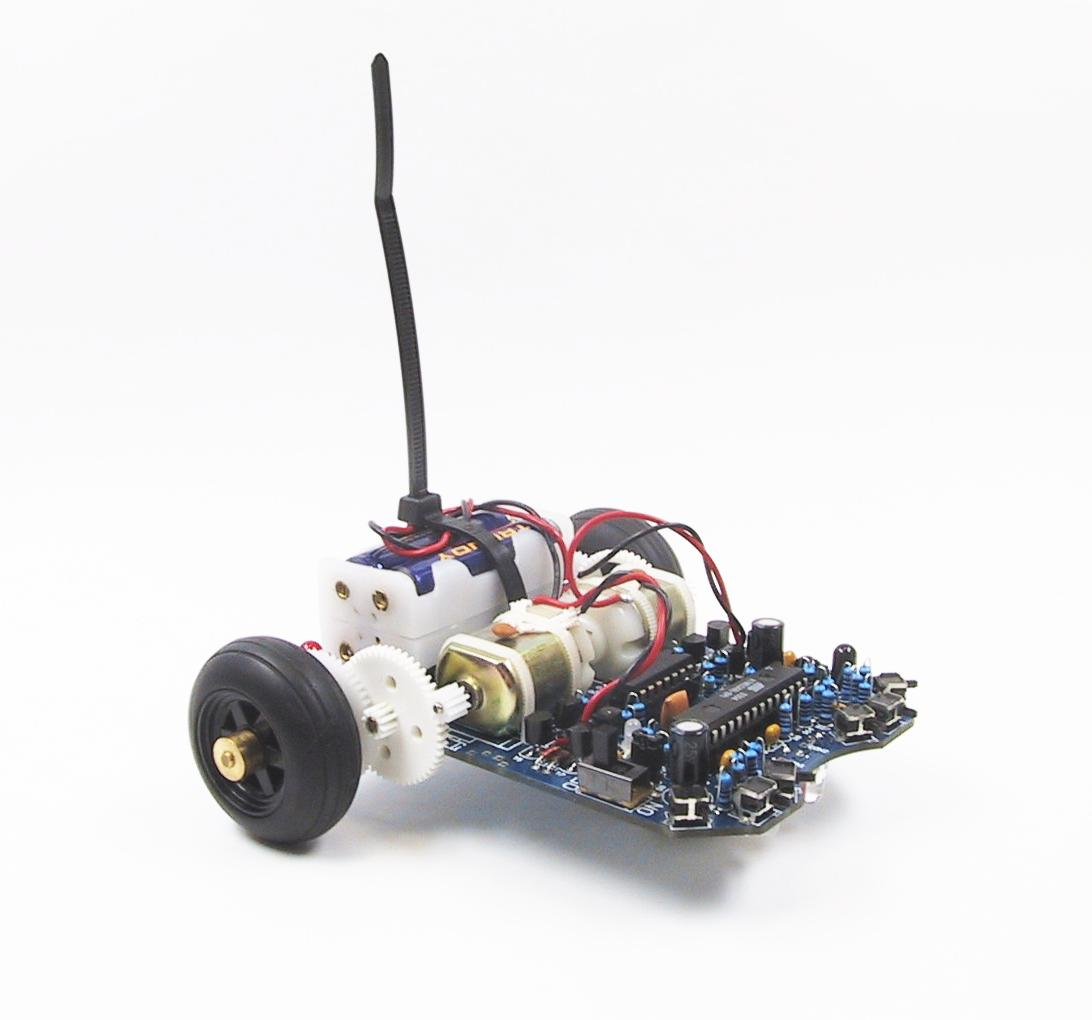
\includegraphics[width=0.5\textwidth]{images/asuro.jpg}
  \caption{Picture of the Asuro (CC-BY-SA Robin Gruber)}
\end{figure}

The Asuro robot is developed by the German Aerospace Center (Deutsches Zentrum für Luft- und Raumfahrt e.V.) in cooperation with Arexx Engineering focused on educational use. Asuros development started in 2004 and is now discontinued. The robot is shipped as a do-it-yourself kit and requires about eight hours build time for a novice. 

Asuro features an eight bit Atmel ATmega8L microcontroller with eight kilobytes of flash memory, 512 bytes of electrical erasable programmable read only memory (short EEPROM) and one kilobytes of static random-access memory (short SRAM). One kilobyte of flash is used for the bootloader which results in seven kilobytes of flash usable for user programs. User programs are uploaded using a infrared serial connection.

Interaction with the environment is realized using two DC motors which can be controlled individually in terms of direction and speed. The robot is stabilized using a half table-tennis ball mounted at the bottom of the robot. Four LEDs are used for displaying the status of the Asuro. The whole system is powered by four AAA batteries or rechargeable batteries mounted in a 2x2 battery case. 

Asuro can sense its environment using different sensors such as two photodiodes which can be used for line-following tasks, six push buttons to detect objects in front of Asuro and two photoelectric sensors to determine the rotation speed of each of Asuros wheels.

\begin{table}[h!]
\centering
\begin{tabular}{p{0.2\textwidth}p{0.2\textwidth}p{0.6\textwidth}}
\toprule
Assessment Criteria    & Rating & Description \\
\midrule
Affordable      & \stars{5}    & Having a price tag of 50 Euro renders the Asuro very affordable in comparison to the 100 Euro limit set. The cost effectiveness is outstanding and features sensors and actuators for basic tasks.     \\
Educational     & \stars{3}     & Asuro features detailed build-instructions in English and German. The guide also includes a tutorial on how to program Asuro in C. Even though there are a lot of opportunities to teach electrical engineering, the available documents do not explain the electrical usage and functional principle of each part. \\
Sustainable       & \stars{4}     & Asuro uses standard components only and features ROHS compliant parts which are free from heavy metals such as lead (PB). A broken Asuro can be easily repaired using the tools which are required to solder it. \\
Extendable & \stars{2}      & Having no free microcontroller pins and no broken out pins, Asuro cannot be considered extendable. There exist some hardware modification in the Asuro community which extend the functionality but require to unsolder/remove some parts.  \\
Trouble-free & \stars{3} & Building Asuro is well documented but some steps may lead to frustration. Mounting the axis using solder is very difficult and may burn the PCB due to the heat emitted in this process. Another frustrating task is to program the robot using the infrared serial connection, since this method is prone to interference. \\
Open-Source & \stars{4} & Asuro was licensed under the DLR-license which is transitioned into a Creative-Commons license model. Everything except the PCB layout files are available for download on the Asuro website.\\
\bottomrule
\end{tabular}
\caption{Asuro evaluation}
\label{tbl:asuro_eval}
\end{table}

All in all the Asuro is a cost effective robot platform suitable for beginners. The lack of extendability and some difficult steps during the build lower the overall good rating to an average of 3.5 stars. 

\subsection{Arduino Robot}
\begin{figure}[h!]
  \centering
  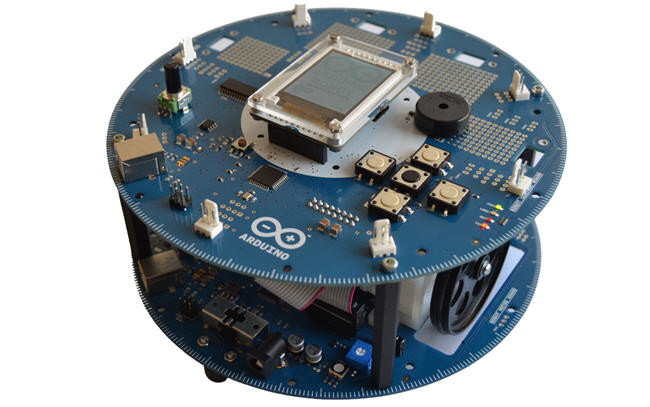
\includegraphics[width=0.5\textwidth]{images/arduinorobot.jpg}
  \caption{Picture of the Arduino Robot}
\end{figure}

The Arduino Robot is the first robot created by the Arduino foundation. It comes preassembled and consists of two different boards: the motor board and the control board. Due to this design, the Arduino robot contains two Atmel ATmega 32U4 microcontroller featuring a clock speed of 16MHz, 32KB of flash memory (of which 28KB can be used for user programs), 2.5KB of RAM and 1KB of EEPROM each.

Each board can be individually programmed using the freely available Arduino IDE having the Robot connected to the computer using an USB cable. The IDE provides a lot of examples for the robot platform and introduces a library for abstract access to the robots functionaly. Power is applied to the system using four rechargeable NIMH-batteries which can be directly recharged on the board by connecting an appropriate power source to the board.

The robot can interact with its environment using movement generated by two controllable DC motors attached to wheels and stabilized using two ball caster. In addition to movement the robot can play sounds using a small speaker on the control board and display text and images on the display mounted on the control board as well. In contrast to the actuators the user can interact with the robot using buttons and several sensors such as infrared sensors for line following tasks or distance measurement.


\begin{table}[h!]
\centering
\begin{tabular}{p{0.2\textwidth}p{0.2\textwidth}p{0.6\textwidth}}
\toprule
Assessment Criteria    & Rating & Description \\
\midrule
Affordable      & \stars{2}    & With a price tag of 189 Euro the Arduino Robot is far above the price limit of 100 Euro. The price for the basic robot is very high compared to its features.\\
Educational     & \stars{3}     & The Arduino robot comes pre-built and therefore lacks the build experience. Learning material for teachers is not provided but a lot of examples and a library to ease programming is provided. Instructions for other Arduino products can be easily adapted to the robot. \\
Sustainable       & \stars{4}     &  The robot integrates charging circuit for the NIMH batteries eliminates the need of a dedicated battery charger and therefore reduces the amount of electrical waste. A small restraint is the choice of components because they cannot be interchanged/repaired by beginners. This is due to the manufacturing process which requires SMD components to be cost effective. Through hole parts would be easier to interchange but require manual assembly which is very expensive.\\
Extendable & \stars{5}      &  Having prototyping areas directly on the control board, the robot can be considered extendable. Moreover connectors for additional sensors are populated all over the robot board making it possible and easy to add sensors without soldering.\\
Trouble-free & \stars{4} & Since the Arduino robot comes pre-assembled and tested in factory, the robot can be called trouble-free. Transportation defects like loose screws can be repaired using household items. The usage is very simple and straight-forward.\\
Open-Source & \stars{3} & Even though it is claimed that the Arduino robot is open-source, not all files required for building the robot are published. The website is missing the PCB design files and includes the schematics only. A software library is available under a open-source license. \\
\bottomrule
\end{tabular}
\caption{Arduino Robot evaluation}
\label{tbl:arduinorobot_eval}
\end{table}

To sum it up the Arduino robot is an extendable robot platform which requires no assembly at all. The integrated battery charging makes it a sustaina ble robot but the high price reduces the overall rating to an average of 3.5 stars.

\subsection{LEGO Mindstorms NXT 2.0}
\begin{figure}[h!]
  \centering
  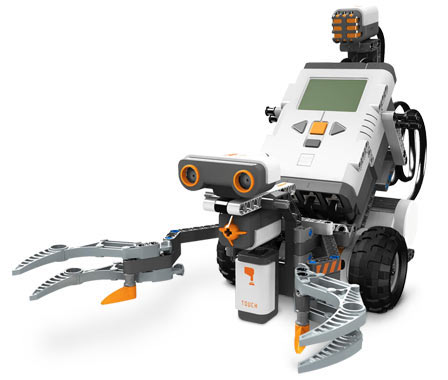
\includegraphics[width=0.5\textwidth]{images/mindstorms.jpg}
  \caption{Picture of the LEGO Mindstorms NXT (from http://www.devoxx.com/)}
\end{figure}

The LEGO Mindstorms NXT 2.0 platform was released by LEGO in 2009 and replaced the first LEGO Mindstorms NXT generation. It is compatible with Lego technic and therefore very flexible/extendable.

LEGO Mindstorms NXT is available in two different kits: the educational kit and a consumer kit. The NXT intelligent brick is the core of the robot platform and contains an 32-bit Atmel ARM7 core with 256KB of Flash memory, 64KB of RAM and supports bluetooth and usb communication to communicate with a host computer. Moreover the brick features a greyscale display, a speaker and four buttons for direct interaction with the brick.

The brick can be powered by using six AA batteries or a rechargeable Lithium-Ion battery with integrated charger which can be separately brought. Sensors and actuators are powered by the brick. A total of four sensors and three actuators can be attached to the brick using flexible cables with a position encoded modular connector.

In the standard kit three continuous rotation servo motors with one degree of accuracy are supplied as well as two touch sensors, one color sensor and an ultrasonic sensor. 

The consumer kit has a price tag of 279 Euro and the education basis set a price tag of 368.99 Euro + 89.24 Euro for the education software.

\begin{table}[h!]
\centering
\begin{tabular}{p{0.2\textwidth}p{0.2\textwidth}p{0.6\textwidth}}
\toprule
Assessment Criteria    & Rating & Description \\
\midrule
Affordable  & \stars{2}    & With a price tag of 279 Euro (retail consumer edition) and 368.99 Euro (education version) the robot is far beyond the price tag of 100 Euro. The amount of sensors and actuators is low compared to the price.\\
Educational & \stars{5}     & LEGO provides a lot of resources for teaching and personal education using the Mindstorms NXT 2.0. Even though the electrical components are not subject, the set can teach a lot of knowledge and even interdisciplinary content. The flexibility of the robot allows the transformation of the robert for a lot of education concern. \\
Sustainable  & \stars{3}     & The Mindstorms NXT 2.0 set cannot be repaired using household items. Nevertheless the components are considered sustainable to a certain extend, since they are designed to be robust and to last a long time.\\
Extendable & \stars{3} & The robot can be extended up to a certain extend. Even though the specification for each interface is public available custom sensors are rare and/or expensive. \\
Trouble-free & \stars{5} & Using the platform is trouble free and easy. The LEGO Mindstorms IDE is intuitional. Support for different programming languages such as Java exist. A huge community and a lot of resources are available.\\
Open-Source & \stars{4} & LEGO open sourced the LEGO Mindstorms NXT brick and moreover the specification for each connector and sensor. The PCB design files and the casing are not open-sourced to prevent unauthorized replicas.\\
\bottomrule
\end{tabular}
\caption{Lego Mindstorms evaluation}
\label{tbl:mindstorms_eval}
\end{table}

All in all the LEGO Mindstorms NXT 2.0 is a great robot platform with a lot of possible applications due to its compability with other LEGO products. The only drawback is the price which is not affordable for everyone.

\subsection{Thymio II}
\begin{figure}[h!]
  \centering
  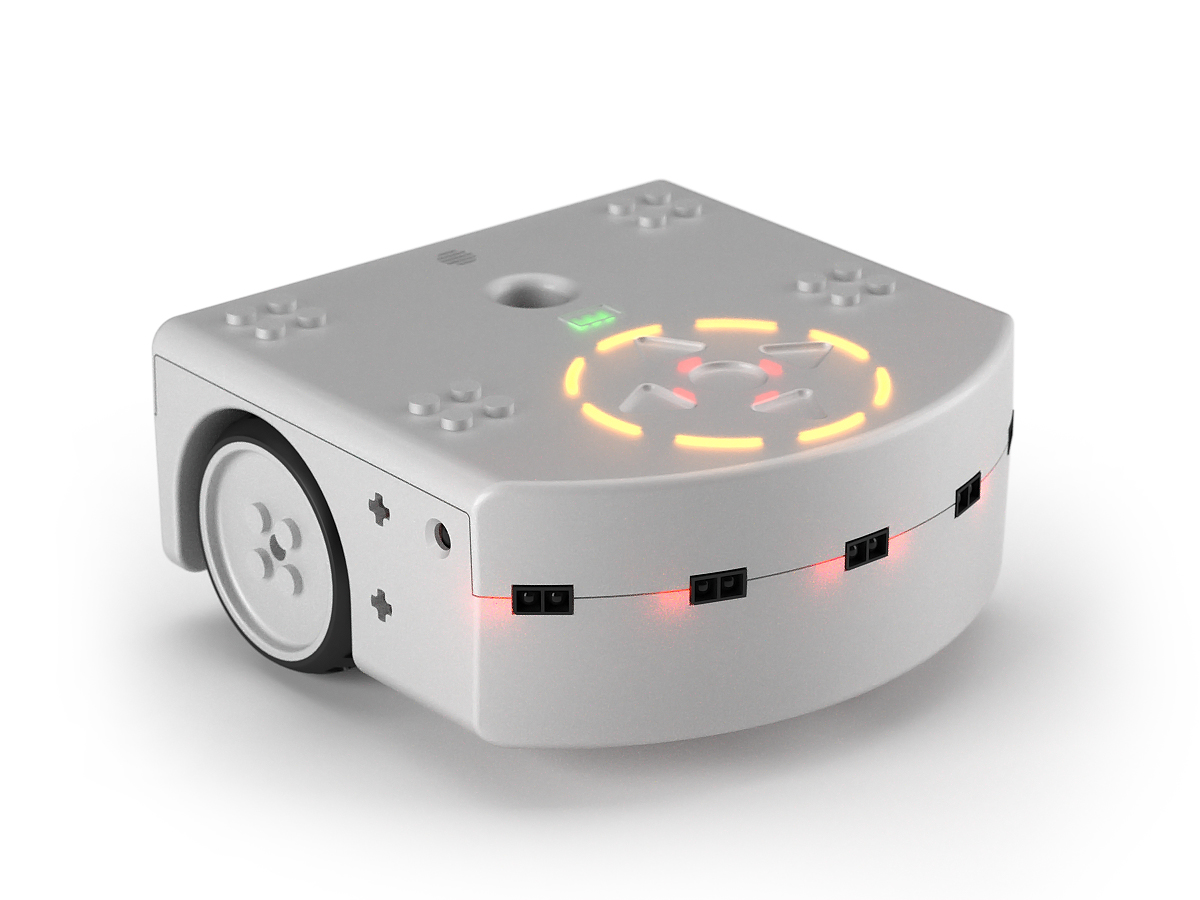
\includegraphics[width=0.5\textwidth]{images/thymioii.jpg}
  \caption{Picture of the Thymio II (from https://aseba.wikidot.com/en:thymio)}
\end{figure}

Thymio II is a robot developed by the Ecole Polytechnique Fédérale de Lausanne and the Ecole Cantonale d'Art de Lausanne for educational purposes. The robot comes preassembled and has a price tag of 99 CHF (plus taxes). It features a 16-bit PIC Microcontroller from Microchip with 128KB Flash, 16KB RAM and a clock Frequency of 8MHz. Programming is archieved using the integrated USB connection

The robot can show its state using several LEDs which illuminate parts of the robots body. It interacts with its environment using two motors and of course the LEDs included. Sensing the environment is archieved using several infrared distance sensors, a microphone, capacitive touch sensors, an accelerometer and a temperature sensor. Data can be stored on a external memory card.

Additional components can be mounted using LEGO compatible mechanical fixation points and an additional Thymio can be attached using the trailer hook. Various support for programming languages exist which adress beginners as well as advanced users.

\begin{table}[h!]
\centering
\begin{tabular}{p{0.2\textwidth}p{0.2\textwidth}p{0.6\textwidth}}
\toprule
Assessment Criteria    & Rating & Description \\
\midrule
Affordable  & \stars{4}    & 99 CHF (without taxes directly from the Ecole Polytechnique Fédérale de Lausanne) is a reasonable price for a robot with this huge amount of features. On retail stores the price is higher due to profit margin.\\
Educational & \stars{3}     & Thymio II does not yet have a repository of educational material only, but it is planned to release such material. The compability with LEGO is a huge bonus, and creates a lot of pplications on which educational problems can be explained and demonstrated.\\
Sustainable  & \stars{3}     & The robot consists of small SMD parts and therefore parts cannot be replaced by the target user group. Materials used are suitable for children and designed to last. The integrated Li-Po battery can be recharged and therefore produces less environmental waste.\\
Extendable & \stars{3} & Except the LEGO compatible fixation points, Thymio II is not extendable without unsoldering components. On the software side, the choice of microcontroller supports a lot of additional program features.\\
Trouble-free & \stars{4} & Thymio II is trouble free since it comes preassembled and the usage is straight forward.\\
Open-Source & \stars{5} & Everything needed to build the robot is licensed under a permissive creative commons license. Program files and libraries are licensed under a LGPL license. Even the CAD files for the plastic mold injection parts are available without a charge.\\
\bottomrule
\end{tabular}
\caption{Thymio II evaluation}
\label{tbl:thymio_eval}
\end{table}

To sum it up the Thymio II platform comes at a great price equipped with a lot of sensors. Its LEGO compatible fixation points are a huge bonus, the license of each aspect of the robot is very permissive. The overall rating of 3.66 stars reflects the huge potential of the platform. Once the educational material is available the platform is considerable as a educational platform.

\section{Case studies}
A robot is built using parts and modules which can be grouped into functional groups like movement, sensors or communication. The goal of each functional group can be achieved in various ways which have to be evaluated using the requirements used in the evaluation of other robot platforms. Some evaluation critera such as the fulfillment of the educational aspect or the open-source aspect may not be suitable for evaluation of single components and therefore left out. The Extendability describes the amount of microcontroller pins where the lesser amount of pins is considered better since this leaves space for extensions. Other difficulties in the evaluation process are dependencies between different modules, e.g. when a sensor has special power requirements. Based on the evaluation the robot will be constructed.
\subsection{Movement}
Movement is the most important feature since it allows the robot to interact with its environment. In contrast to a stationary robot, a moving robot can interact with a wider area but requires battery power or similar mobile energy sources. Different approaches for robot movement exist which will be part of critical evaluation.

There exist wheeled, legged, flying, swimming, diving and much more robot movement types. Wheeled robots are common since their mechanic principle is rather simple, cheap and easy to implement and control. Therefore other mentioned movement techniques except wheeled robots are not part of the evaluation.

Typically robots have two wheels and a ball caster which prevents the robot from falling over. A ball caster acts as a third unidirected wheel with reduced friction. Alternatively four wheels and a steering mechanism or three wheels using omniwheels can be used. All types of wheeled robots can move in flat terrain and tolerate slight uneven surfaces. The outdoor usage is limited.
\subsubsection{Wheeled with two DC motors}
DC motors (direct current motors) are a cheap solutions for driving wheels. Usually a gear box is required to reduce the motor speed in favor of torque. Controlling the direction (forward and backward) requires the ability to switch the direction of the current flow. This is usally archieved using a H-bridge which can be found in as an integrated circuit or build using four electrical switches. 

There exist integrated circuits which provides two H-bridges combined in one component which allow the control of steering beneath the control of direction. Speed control is controlled by an external PWM (pulse-width-modulation) source.

%TODO Image of gearbox motor

In terms of cost effectiveness a solution with two wheels powered by a DC motor each performs well. A DC motor with integrated gearbox (see figure @TODO) is available for 5.5 USD, the plastic wheel costs 3.5 USD, a motor driver such as the L293 costs about 3.5 USD rendering a total cost of 21.5 USD per robot. In addition speed sensors for each of the wheels are needed since the motors do not have exactly the same speed. Without speed control the robot cannot drive straight forward.

The mentioned gearbox cannot be repaired once broken and should be replaced rather than repaired. Moreover it is unclear which materials are used in the plastic parts and whether they can be recycled. Mounting and controlling the motors is trouble free and requires at least six microcontroller pins as one can see in the following table.

\begin{table}[h!]
\centering
\begin{tabular}{p{0.15\textwidth}p{0.15\textwidth}p{0.5\textwidth}}
\toprule
Pin count & Pin type & Description \\
\midrule
2 & PWM  & Motor speed control using pulse-width-modulation.\\
4 & GPIO & Direction control and steering control using a 4-bit (16 combinations) pattern.\\
\bottomrule
\end{tabular}
\caption{DC motor microcontroller pin usage}
\label{tbl:dc_pin}
\end{table}

When using a shift register for setting the four GPIO inputs of the motor driver, the pin count on the microcontroller can be reduced to three pins (Clock, Serial Data, Enable).  A single shift register can provide eight GPIO port and can be chained.


\subsubsection{Wheeled with two Stepper motors}
Stepper motors are basically DC motors with more coils. In stepper motors the full rotation is divided into a number of equal steps which can be separately controlled. The motor can step forward, backward or hold the current position with huge torque. Stepper motors are usually shipped within a gear box which reduces steps much further to gain higher precision and torque. 
In typical applications stepper motors are driven by a dual H-bridge or darlington arrays attached to shift registers. The latter method is very cost effective but limited in current supply, the first method utilized a motor driver such as the L293 per stepper.

Stepper motors are availble for about 5 USD (in the USA\footnote{http://www.adafruit.com/products/858}). Two stepper motors are needed to drive the robot, an additional ball caster is needed to stabilize the movement. As mentioned in the forehand the cost of driving a stepper motor can be reduced using a shift register such as the 74HC595 in combination with a darlington array such as the ULN2803. Costs for this solution are about 12 USD where the stepper motors cost 10 USD, and the integrated circuits about 2 USD.

The pin usage on the microcontroller using the shift register is as follows:

\begin{table}[h!]
\centering
\begin{tabular}{p{0.15\textwidth}p{0.15\textwidth}p{0.5\textwidth}}
\toprule
Pin count & Pin type & Description \\
\midrule
1 & GPIO & Clock which clocks the serial data. Not time critical due to the design of a shift register.\\
1 & GPIO & Serial data in which sets the bit pattern.\\
1 & GPIO & Chip enable which enables the shift register output.\\
\bottomrule
\end{tabular}
\caption{Shift register microcontroller pin usage}
\label{tbl:74hc595_pin}
\end{table}

Since shift registered are chainable, several stepper motors can be controlled using three pins only. A typical 74HC595 shift register has a settle time of 13 nanoseconds which allows 76900 switch cycles per second. For an eight bit shift register about 9600 full state changes can be performed, each additional shift register reduces the amount by half.

If a stepper motor gets broken, it can be easily replaced using the same model of stepper motor. Since the wheel is not part of the stepper motor, the old wheel can be replaced easily.
\subsubsection{Omniwheels}
Omniwheels/Mecanum wheels are the most flexible way of moving using wheels. Omniwheels are a special form of wheels which allow the movement in any direction having three independently moveable wheels. It requires three motors (typically DC motors) with direction control and optional speed control.

\begin{figure}[h!]
  \centering
  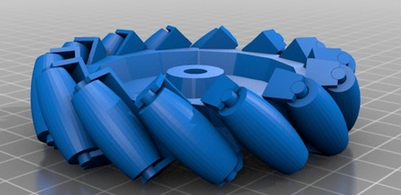
\includegraphics[width=0.5\textwidth]{images/mecanum.png}
  \caption{Screenshot of a mecanum wheel 3D model (from http://www.thingiverse.com/thing:2318)}
\end{figure}

Integrating omni wheels into the robot plattform reduces the need of ball caster for stabilization but increases costs due to the need of an additional motor and motor controller. Moreover omni wheels itself have a price tag of 4 USD each which sums up to 12 USD for the wheels, three motors for 5.5 USD and two motor drivers for 3.5 USD each. This renders a cost of 35.5 USD plus the speed sensors which adds to even more. 

The pin usage is similar to the pin usage of wheeled robots with two DC motors. The control is more difficult since the control scheme is complex due to the movement vectors as shown in the figure \ref{fig:omnicontrol}.

\begin{figure}[h!]
  \centering
  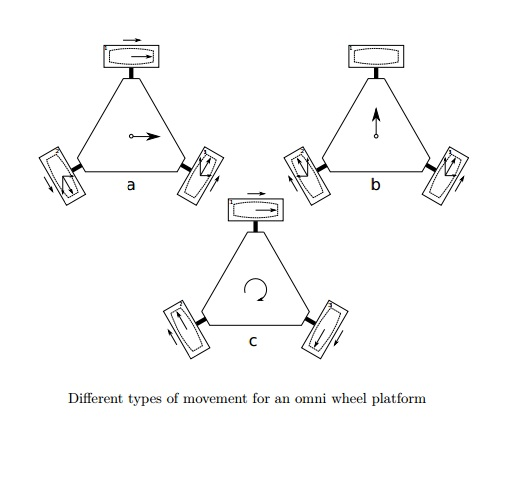
\includegraphics[width=0.5\textwidth]{images/omniwheel.jpg}
  \caption{Control scheme of a omni wheel (from http://commons.wikimedia.org/wiki/File:Omni\_wheel\_control.jpg)}
  \label{fig:omnicontrol}
\end{figure}


\subsubsection{Conclusion}
All in all a solution using stepper motors with darlington array connected to shift registers is the most cost-effective solution. It provides the necessary functions and complies to the evaluation aspects such as the educational potential. Its usage is rather trouble free when apropriate libraries for motor control are provided.

\subsection{Sensors}
Sensors are important to make the robot sense its environment. Sensing the environment enables interaction such as obstacle avoidance, finding objects or following lines. Connecting sensors to a microcontroller can be done in various ways using various protocols. Different protocols require a different amount of microcontroller pins. Dependening on the sensor technology more or less computing time is needed to evaluate the sensors value.  

\subsection{IR Reciever}
Infrared Reciever are special photodiodes which react on infrared light with a base frequency of 38kHz. To ease the use of IR recievers with microcontrollers, the photodiode in the IR reciever provides a near binary square voltage waveform instead of rising voltages. The cost of such a reciever is about 0.3USD.

IR recievers are widely used in remote control applications such as televisions and remote controlled toys. Sending a signal requires a LED which emits light in the infrared spectrum. Cheap multipurpose remotes (about 1 USD) can be used to control own applications. Infrared beacons which steadily send a signal can be used to give a robot information on its current location.

Attaching a reciever to a microcontroller requires a single input pin which can be either a digital pin or a pin internally attached to an ADC. In terms of cost effectiveness and education potential IR recievers are a must have sensor. Under the premise that library for infrared readings exist, the sensor is easy to use and trouble free.

\subsection{Ultrasonic Distance Sensor}
Ultrasonic distance sensors sense distance between the sensor and an object in the visible area of the sensor. In case of ultrasonic sensors the visible area is the area where the echo spreads. By counting the time between the signal and the reflection the distance can be calculated using the speed of sound (340.29 m / s at sea level). 

The price for an ultrasonic distance sensor is very low, cheap versions with a range between 1 and 255 centimeters start at about 1.5 USD. Interfacing the sensor requires two microcontroller pins - one for triggering the echo and another one for reading back the distance value. The trigger pin can be a generic purpose input/output pin, the sense pin must be attached to a pin which provides an analog to digital converter.

A typical application for ultrasonic distance sensor is obstacle avoidance. By mounting the sensor on a servo motor the visible area can be increased which allows better navigation due to enhanced obstacle avoidance possibilities. 

\subsection{Accelerometer}
Accelerometers can sense acceleration on one or more axis. This can be used to determine the speed of the robot or the direction in which the robot accelerates (which can be used to determine whether the robot falls/is lifted up). 

Interfacing accelerometer is often done using serial protocols like SPI (Serial Periphal Interface), UART (Universal asynchronous receiver/transmitter) or I2C (Inter-Integrated Circuit). A affordable accelerometer with included gyroscope (evaluated in the section below) is the MPU-6050. It has a price tag of 3 USD and is usually sold on a breakout-board due to its small QFN (quad-flat no-leads) package which is hard to solder manually. 

The MPU-6050 can be interfaced using various protocols, but I2C is the most common way to do so and requires two input/output pins only using software-based I2C or two I2C hardware pins. Libraries with permissive license exist which ease the use of the accelerometer. For advanced usage scenarios a integrated DMP (Digitial Motion Processor) can process raw values and interface additional sensors like a compass.
\subsection{Gyroscope}
Gyroscopes are used to determine the orientation. Applications for gyroscopes are balancing and position calculation (usually in combination with an accelerometer). Integrated circuits such as the MPU-6050 mentioned before usually combine a gyroscope and an accelerometer into one single device.

The educational potential of a gyroscope/accelerometer is excellent, since interaction with a robot can be directly visualized. It can introduce the user to concepts of orientation and force by interacting with the robot. Advanced users can use the sensor to determine the position in of the robot based on a known starting point or lifting/falling detection.

As mentioned in the previous section the MPU-6050 is easily interfaced using various protocols of which I2C is the common way.
\subsection{Compass}
A compass allows the robot to sense its orientation relative to the magnetic field of the earth. Technically speaking a integrated circuit providing measurement of the magnetic field of the earth are a special form of magnetometers.



\subsubsection{Conclusion}
\subsection{Communication}
Communication between robots or between the robot is essential to widen the application possibilities. When the robot is connected to a computer it gets much more processing power to solve complicated problems; when robots can communicate with each other tasks can be solved collaboratively.

\subsubsection{Infrared}
Infrared based data transfer is widely used in remote control application where a small amount of data is transferred. Infrared communication is easily interfered by other infrared signals. This limits the data rate since error correction mechanisms must be implemented.

When using infrared signals only one robot can send at a time which requires collision detection. The hardware requirements for infrared transmissions are ver low, only a infrared reciever and a infrared LED is required which sums up to a total of 0.5 USD. The infrared reciever and the infrared LED require one free GPIO pin on the microcontroller each.

Since a lot of effort is needed to make the connection stable, this solution is not trouble free, although techniques to stabilize communication have educational potential.

\subsubsection{RFM12}
\subsubsection{Bluetooth}
\subsubsection{NRF24L01}

\subsection{Microcontroller}

\subsubsection{ATmega328p}
\subsubsection{ATmega32U4}

\subsection{Power Supply}
\subsubsection{Nickel-metal hydride batteries}
\subsubsection{Lithium Polymer batteries}

\section{Robot Construction}



\nocite{*}
\printbibliography
\addcontentsline{toc}{part}{References}
\end{document}
